\documentclass[border=0.25cm]{standalone}

\usepackage{tikz}
% \usepackage{fouriernc}

\begin{document}

  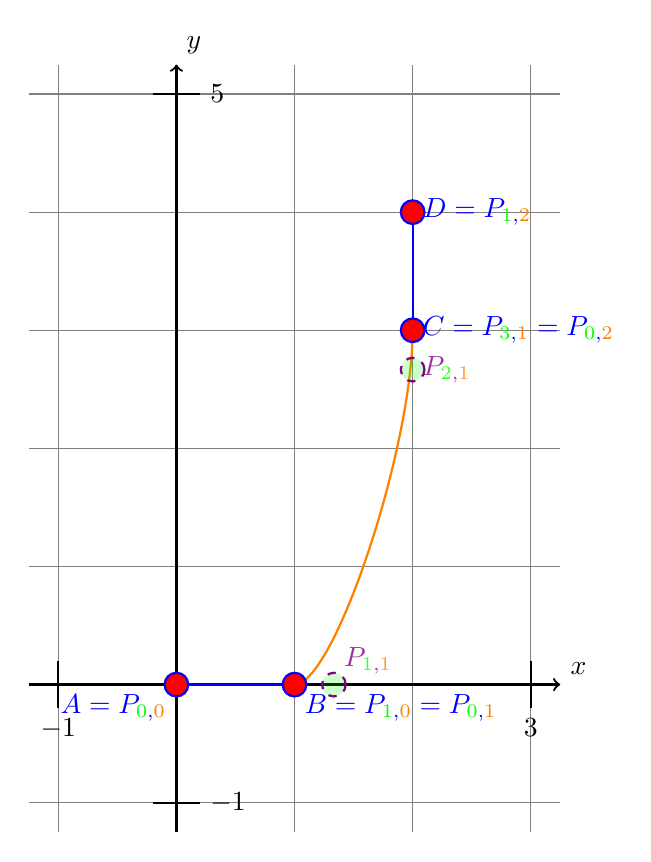
\begin{tikzpicture}[scale=1.5]

    \draw[gray] (-1.25, -1.25) grid (3.25, 5.25);

    % x-axis
    \draw[thick, black, ->] (-1.25, 0) -- (3.25, 0)
      node[anchor=south west] {$x$};

    % x-axis tick marks
    \foreach \x in {-1, 3}
      \draw[thick] (\x, 0.2) -- (\x, -0.2)
        node[anchor=north] {\(\x\)};

    % y-axis
    \draw[thick, black, ->] (0, -1.25) -- (0, 5.25)
      node[anchor=south west] {$y$};

    % y-axis tick marks
    \foreach \y in {-1, 5}
      \draw[thick] (-0.2, \y) -- (0.2, \y)
        node[anchor=west] {\(\y\)};

    % graph of function

    % \draw[thick, blue, ->] (-5, 4) .. controls (-5, 2) and (-4, 2) .. (-3, 2)
    %   .. controls (-2.1, 2) and (-2.1, 3) ..
    %   (-2.1, 5.25);

    % \draw[thick, dashed, red] (-2, -5.25) -- (-2, 5.25);

    \draw[thick, orange, -] (1, 0) ..
    controls (4/3, 0) and (2, 2) .. (2, 3);

    \draw[thick, blue] (0, 0) -- (1, 0);
    \draw[thick, blue] (2, 3) -- (2, 4);

    \draw[thick, blue, fill=red] (0, 0) circle (1mm) node[anchor=north east] {$A=P_{\textcolor{green}{0},\textcolor{orange}{0}}$};

    \draw[thick, blue, fill=red] (1, 0) circle (1mm) node[anchor=north west] {$B=P_{\textcolor{green}{1},\textcolor{orange}{0}}=P_{\textcolor{green}{0},\textcolor{orange}{1}}$};
    \draw[thick, blue, fill=red] (2, 3) circle (1mm) node[anchor= west] {$C=P_{\textcolor{green}{3},\textcolor{orange}{1}}=P_{\textcolor{green}{0},\textcolor{orange}{2}}$};
    \draw[thick, blue, fill=red] (2, 4) circle (1mm) node[anchor= west] {$D=P_{\textcolor{green}{1},\textcolor{orange}{2}}$};

    \draw[thick, violet, dashed, fill=green, fill opacity=0.2] (2, 8/3) circle (1mm) node[anchor= west, fill opacity=0.8] {$P_{\textcolor{green}{2},\textcolor{orange}{1}}$};
    \draw[thick, violet, dashed, fill=green, fill opacity=0.2] (4/3, 0) circle (1mm) node[anchor= south west, fill opacity=0.8] {$P_{\textcolor{green}{1},\textcolor{orange}{1}}$};


    % \draw[thick, blue, fill=blue] (-3, -3) circle (1mm);

    % \draw[thick, blue, fill=white] (2, -4) circle (1mm);

    % \draw[thick, blue, fill=blue] (2, 4) circle (1mm);

    % \draw[thick, blue, fill=blue] (5, -2) circle (1mm);


  \end{tikzpicture}
\end{document}